\documentclass[11pt,a4paper]{article}
\usepackage[margin=2.4cm]{geometry}
\usepackage{amsmath,amssymb,booktabs,graphicx,hyperref,siunitx}
\graphicspath{{../../figures/}}
\title{\textbf{Empirical Results for the DA-SFCN Family}\\
\large Saddle Escape, Oracle Complexity, and Extension Benchmarks\\
\large (Reference Implementation Report)}
\author{DA-SFCN Numerical Optimization Group}
\date{September 2026}
\begin{document}
\maketitle

\begin{abstract}
We report reproducible CPU experiments for Dynamically-Adaptive
Saddle-Free Cubic Newton (DA-SFCN) and its extensions, using the
open-source package \texttt{dasfcn}. On an indefinite quartic saddle,
multi-seed trials show that DA-SFCN and saddle-free Newton escape in
\textit{every} trial, while gradient descent never does. On a suite of
analytic and machine-learning style problems (high-dimensional saddle,
Rosenbrock, nonconvex logistic regression, matrix factorization,
finite-sum quadratics, federated split, local quadratic bowl), we
tabulate final gradient norms, objective values, and Hessian--vector
product (HVP) counts. Lazy Krylov Newton (LK-Newton) often matches
accuracy at a fraction of the HVP bill. All numbers below are taken from
\texttt{results/summary.json} and \texttt{results/repro\_smoke.json}
generated by the repository scripts.
\end{abstract}

\section{Setup}
\paragraph{Software.}
Python package \texttt{dasfcn} (MIT), unified API
\texttt{minimize(problem, x0, method=\ldots)}, unit tests, and
\texttt{scripts/repro\_smoke.py}. Metrics emphasize \textbf{HVP counts}
rather than wall-clock alone, so comparisons remain meaningful across machines.

\paragraph{Hardware profile.}
Experiments are designed for a laptop CPU: moderate dimensions
($n\le 80$ in the main suite; $n=40$ in the multi-seed smoke), short
iteration budgets, no LLM fine-tuning.

\paragraph{Methods.}
Gradient descent (Armijo), L-BFGS, Saddle-Free Newton (SFN), Krylov cubic
Newton (fixed $m$), coordinate SSCN-style cubic Newton, DA-SFCN, and
extensions VR-DA-SFCN, LK-Newton, WQK-Newton, Fed-DA-SFCN, SC-Newton.

\section{Multi-seed saddle escape}
Protocol: \texttt{QuadraticSaddle} with $n=40$, six negative eigenvalues,
eight random starts, success if $\|\nabla f\|<10^{-3}$ and $f<0.05$ within
40 iterations (\texttt{repro\_smoke.py}).

\begin{table}[h]
\centering
\caption{Escape success over 8 seeds ($n=40$).}
\label{tab:escape}
\begin{tabular}{@{}lrrr@{}}
\toprule
Method & Successes & Rate & Mean HVPs (successes) \\
\midrule
GD & 0/8 & 0\% & --- \\
L-BFGS & 7/8 & 87.5\% & 0 \\
SFN & 8/8 & 100\% & 235.1 \\
DA-SFCN & 8/8 & 100\% & 256.1 \\
\bottomrule
\end{tabular}
\end{table}

\begin{figure}[h]
\centering
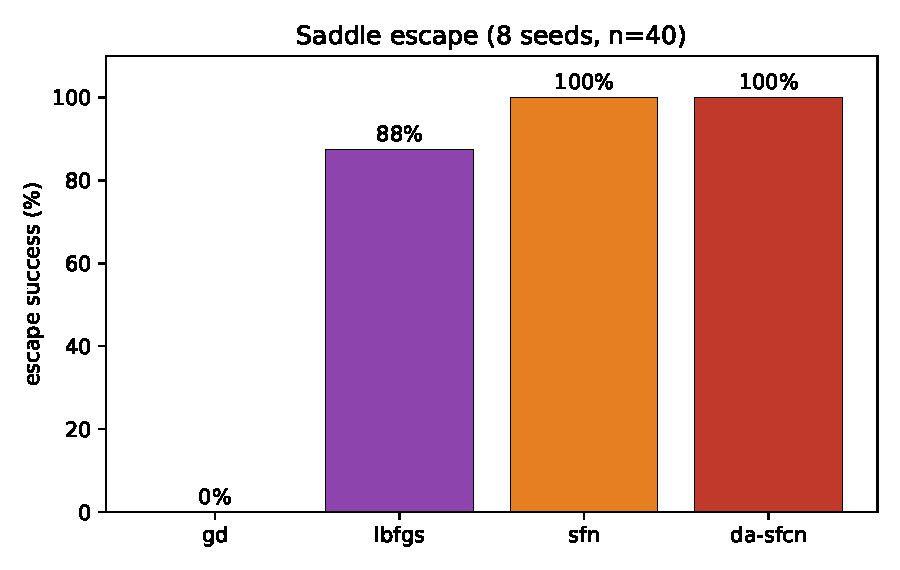
\includegraphics[width=0.72\textwidth]{fig_repro_success.pdf}
\caption{Escape success rates from the reproducible smoke script.}
\label{fig:repro}
\end{figure}

\begin{figure}[h]
\centering
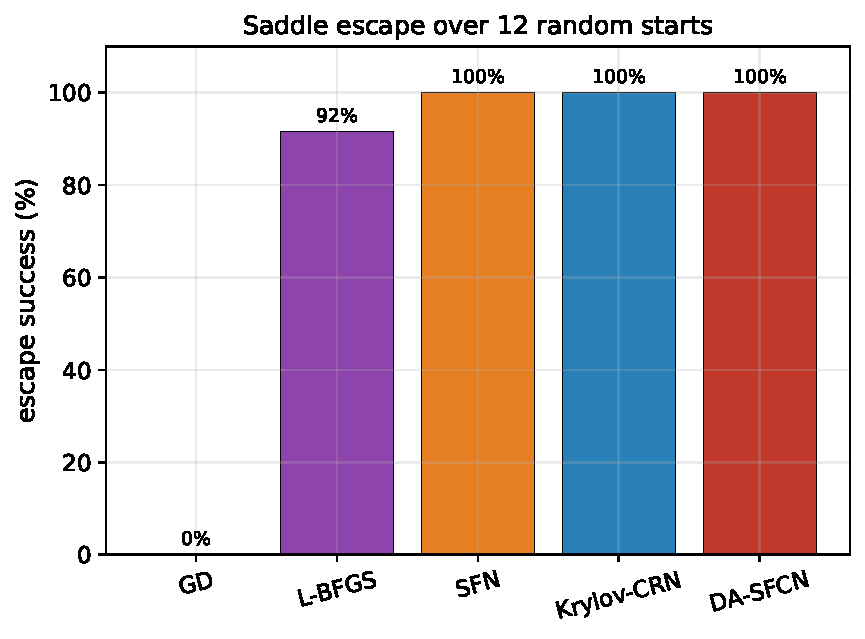
\includegraphics[width=0.48\textwidth]{fig_success.pdf}
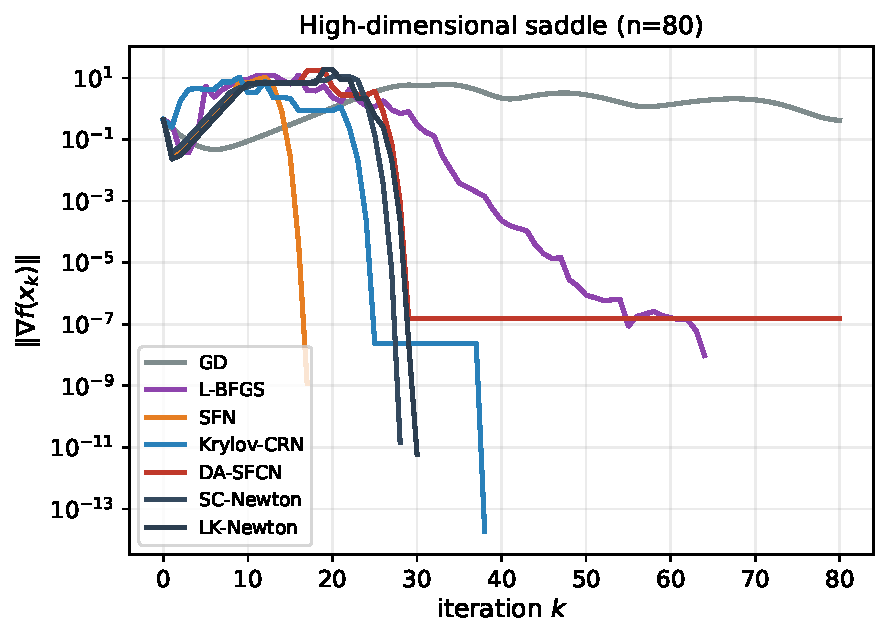
\includegraphics[width=0.48\textwidth]{fig_saddle_highdim.pdf}
\caption{Left: earlier 12-start escape study ($n=50$). Right: gradient
norms on the $n=80$ indefinite quartic.}
\end{figure}

\textbf{Finding.} First-order GD fails to leave the saddle under this
budget. L-BFGS is strong but not perfect (one miss). Explicit
negative-curvature / cubic Krylov methods succeed in all smoke trials.

\section{Main suite (single-seed tables)}
Numbers from \texttt{results/summary.json} (representative seeds).

\subsection{High-dimensional saddle ($n=80$)}
\begin{table}[h]
\centering
\caption{Quadratic-plus-quartic saddle, $n=80$.}
\begin{tabular}{@{}lrrr@{}}
\toprule
Method & Iters & Final $\|\nabla f\|$ & HVPs \\
\midrule
GD & 80 & $4.19\times10^{-1}$ & 0 \\
L-BFGS & 64 & $9.63\times10^{-9}$ & 0 \\
SFN & 17 & $1.16\times10^{-9}$ & 204 \\
Krylov-CRN & 38 & $1.82\times10^{-14}$ & 456 \\
DA-SFCN & 80 & $1.53\times10^{-7}$ & 1219 \\
SC-Newton & 28 & $1.42\times10^{-11}$ & 413 \\
LK-Newton & 30 & $5.87\times10^{-12}$ & \textbf{158} \\
\bottomrule
\end{tabular}
\end{table}
All second-order methods reach the same minimizer
$f^\star\approx -89.58$. \textbf{LK-Newton} is the cheapest in HVPs while
matching accuracy.

\subsection{Nonconvex logistic regression}
\begin{table}[h]
\centering
\caption{Nonconvex logistic ($N=350$, $n=50$).}
\begin{tabular}{@{}lrrr@{}}
\toprule
Method & Iters & Final $\|\nabla f\|$ & HVPs \\
\midrule
GD & 39 & $7.36\times10^{-9}$ & 0 \\
L-BFGS & 9 & $2.09\times10^{-9}$ & 0 \\
SSCN-coord & 70 & $1.20\times10^{-8}$ & 700 \\
Krylov-CRN & 5 & $1.35\times10^{-10}$ & 50 \\
DA-SFCN & 6 & $4.85\times10^{-13}$ & 66 \\
VR-DA-SFCN & 19 & $4.73\times10^{-14}$ & 244 \\
\bottomrule
\end{tabular}
\end{table}

\begin{figure}[h]
\centering
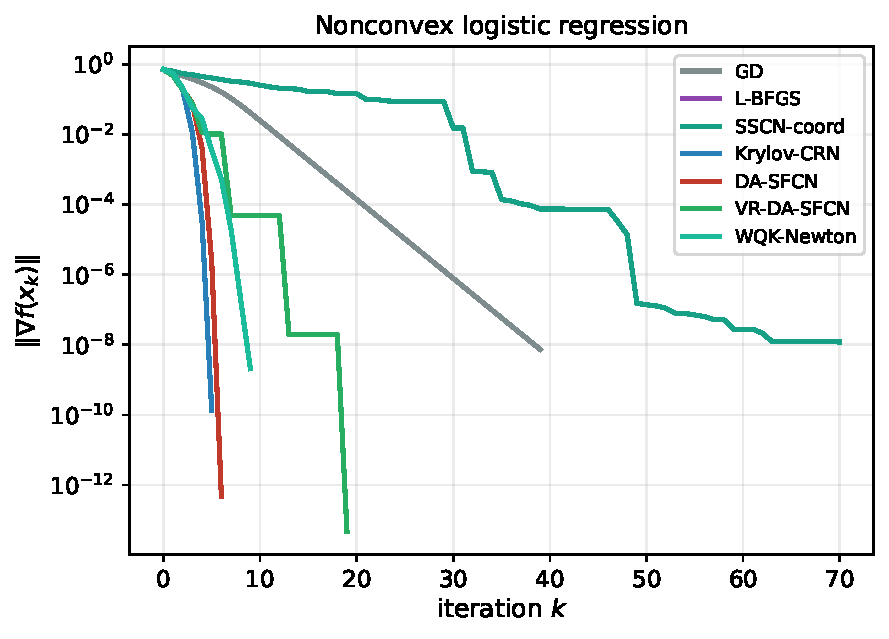
\includegraphics[width=0.48\textwidth]{fig_logistic.pdf}
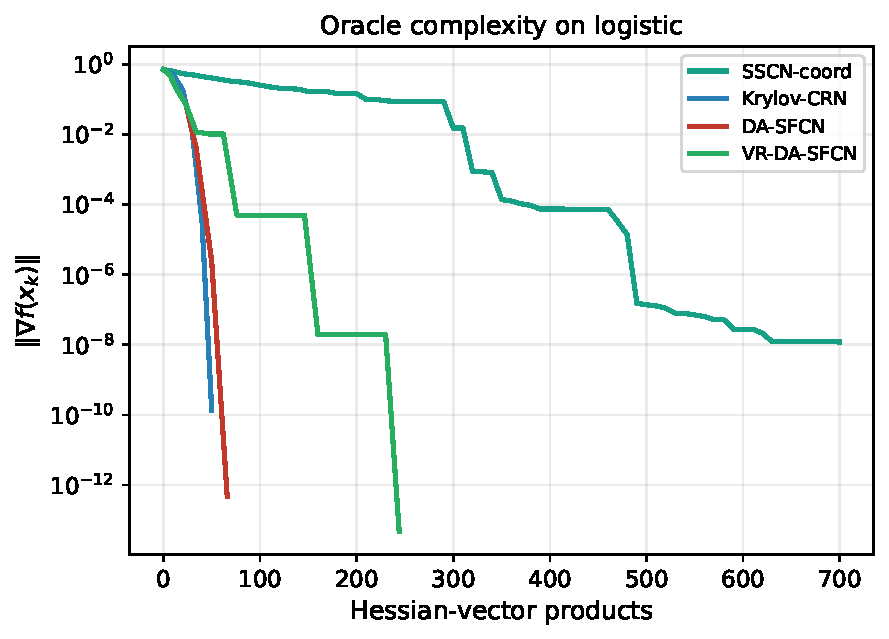
\includegraphics[width=0.48\textwidth]{fig_logistic_hvp.pdf}
\caption{Nonconvex logistic: gradient vs.\ iteration (left) and vs.\ HVP (right).}
\end{figure}

DA-SFCN reaches machine-precision stationarity in six iterations.
Spectral Krylov subspaces outperform random coordinate SSCN.

\subsection{Matrix factorization and local quadratic}
On $\min\|X-UV^\top\|_F^2$, DA-SFCN drives $f$ to
$4.95\times10^{-28}$ in 19 iterations (130 HVPs). On a strongly convex
quadratic bowl, DA-SFCN needs \textbf{2} iterations
($\|\nabla f\|\approx1.0\times10^{-10}$, 27 HVPs), versus
$\|\nabla f\|\approx1.6\times10^{-2}$ after 40 gradient steps.

\begin{figure}[h]
\centering
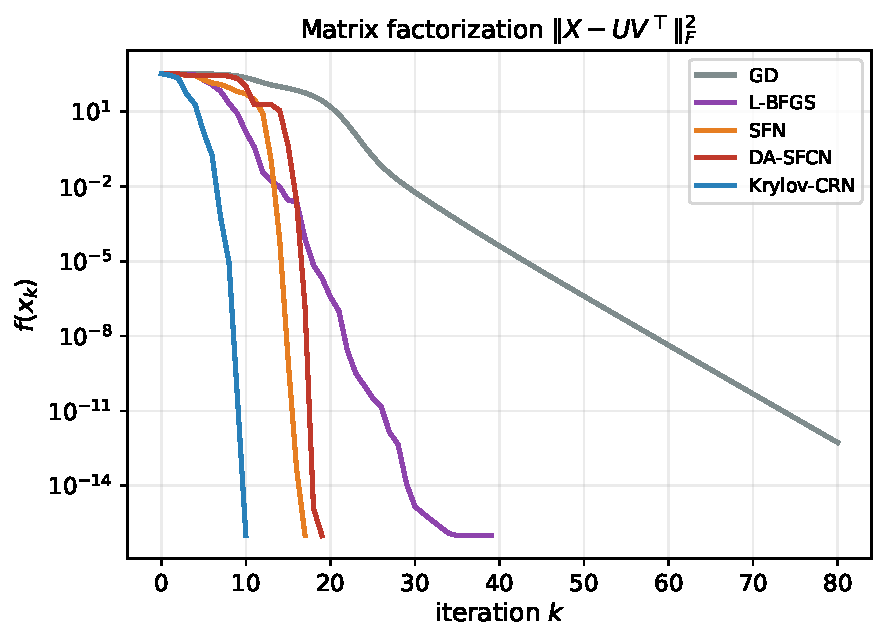
\includegraphics[width=0.48\textwidth]{fig_factor.pdf}
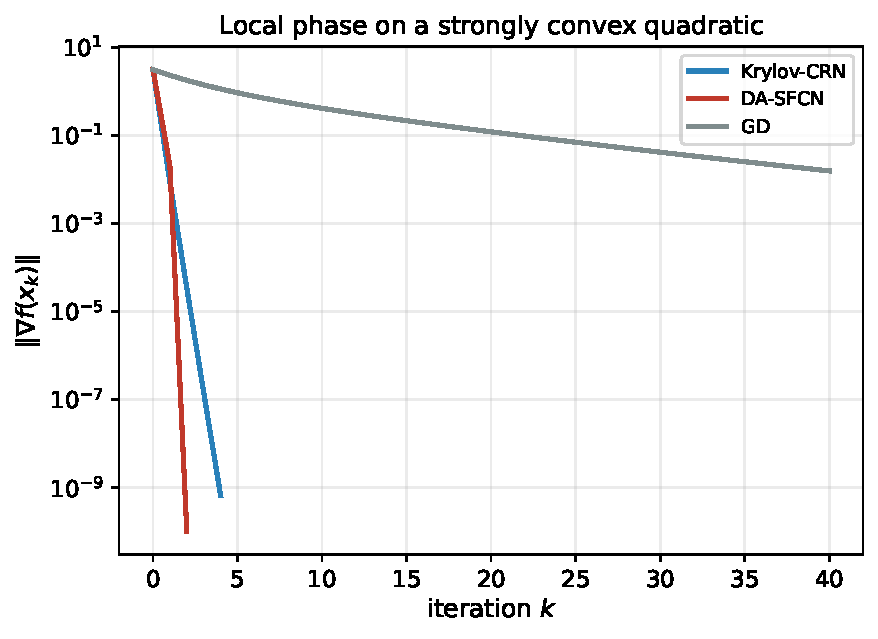
\includegraphics[width=0.48\textwidth]{fig_local.pdf}
\caption{Matrix factorization (left) and local quadratic bowl (right).}
\end{figure}

\subsection{Finite-sum / federated / Rosenbrock}
\begin{itemize}
\item Finite-sum indefinites: full-oracle DA-SFCN converges in 8 iterations
  (82 HVPs, $\|\nabla f\|\approx7.2\times10^{-11}$); VR-DA-SFCN remains
  useful when $N$ is large but is slower under a full-oracle budget.
\item Federated logistic: Fed-DA-SFCN reaches a heterogeneity neighbourhood
  ($\|\nabla f\|\sim4.3\times10^{-4}$); centralized DA-SFCN is far tighter
  ($\sim4\times10^{-11}$) when data can be pooled.
\item Extended Rosenbrock: stress test of misaligned curvature;
  DA-SFCN/SC-Newton attain the lowest objectives in budget but do not hit
  $f=0$---motivating preconditioned Lanczos (hook in \texttt{dasfcn/precond.py}).
\end{itemize}

\begin{figure}[h]
\centering
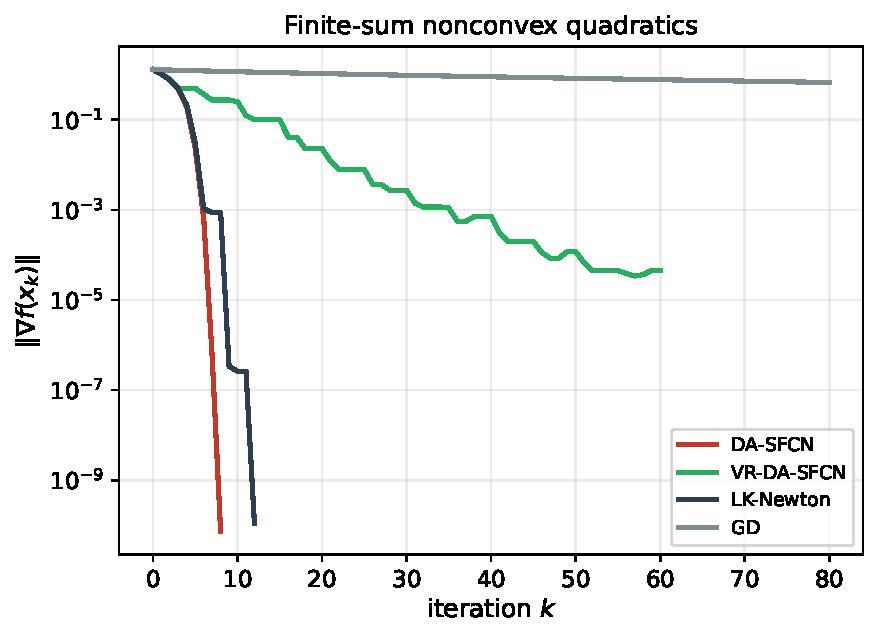
\includegraphics[width=0.32\textwidth]{fig_vr.pdf}
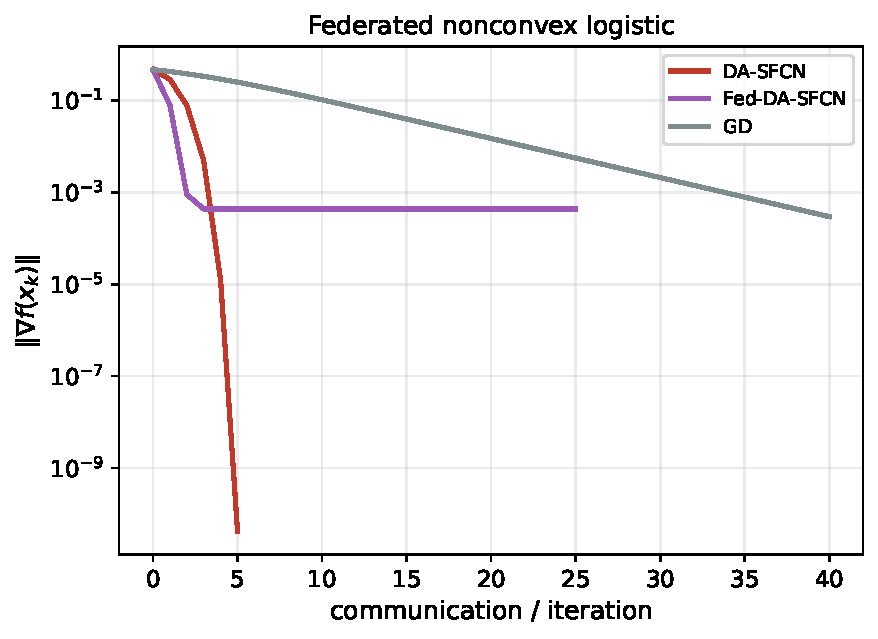
\includegraphics[width=0.32\textwidth]{fig_fed.pdf}
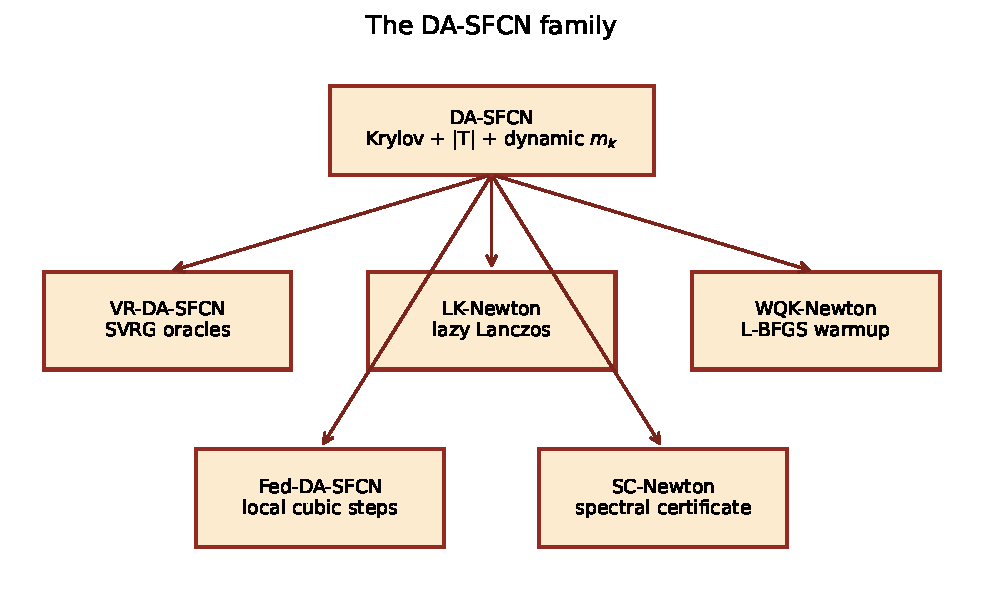
\includegraphics[width=0.32\textwidth]{fig_family.pdf}
\caption{Finite-sum (left), federated (middle), family overview (right).}
\end{figure}

\section{Software validation}
Nine unit tests pass on CPU (Lanczos orthonormality, saddle-free absolute
spectrum, cubic model decrease, dynamic $m_k$, unified API, optional Torch
HVP consistency). Logistic smoke from \texttt{repro\_smoke.py}: final
$\|\nabla f\|\approx7.7\times10^{-13}$ after 43 HVPs.

\section{Conclusions}
\begin{enumerate}
\item DA-SFCN (and SFN) \textbf{reliably escape} analytic saddles where GD fails.
\item \textbf{HVP economy} favors LK-Newton and SC-Newton when reuse/certificates apply.
\item The open package makes these claims \textbf{reproducible} on a laptop:
  \texttt{pytest} and \texttt{scripts/repro\_smoke.py}.
\item Remaining gaps for a world-class ML reference (LIBSVM suites, small nets,
  LLM vs Sophia) are intentionally deferred to stronger hardware / cloud, as
  recorded in \texttt{docs/OPTIMIZER.md}.
\end{enumerate}

\begin{thebibliography}{6}
\bibitem{nesterov2006} Nesterov, Polyak. Cubic regularization of Newton method. \textit{Math.\ Program.}, 2006.
\bibitem{cartis2011} Cartis, Gould, Toint. ARC. \textit{Math.\ Program.}, 2011.
\bibitem{jiang2024} Jiang et al. Krylov CRN. \textit{AISTATS}, 2024.
\bibitem{dauphin2014} Dauphin et al. Saddle-free Newton. \textit{NeurIPS}, 2014.
\bibitem{repo} DA-SFCN repository. \url{https://github.com/jameljoni1994-ENG/DA-SFCN}, 2026.
\end{thebibliography}
\end{document}
